\documentclass[journal]{IEEEtran}
\IEEEoverridecommandlockouts
\usepackage{cite}
\usepackage{amsmath,amssymb,amsfonts}
\usepackage{graphicx}
\usepackage{textcomp}
\usepackage{xcolor}
\usepackage{booktabs}
\usepackage{multirow}
\usepackage{url}
\usepackage{balance}
\usepackage{hyperref}

\graphicspath{{figures/}}

\begin{document}

\title{CAMAS: A Carbon-Aware Multi-Agent System for\\
Energy-Efficient LLM Orchestration}

\author{\IEEEauthorblockN{Praveen Raj}
\IEEEauthorblockA{\textit{Department of Computer Science}\\
\textit{[Institution Name]}\\
[City, Country]\\
[email@institution.edu]}
}

\maketitle

% ============================================================
\begin{abstract}
Agentic Artificial Intelligence has pushed large language model (LLM)
applications beyond single-pass inference into complex, multi-step autonomous
workflows. While this autonomy improves task completion capability, it
introduces significant and largely unmeasured computational overhead at the
orchestration layer. Existing Green AI and carbon-aware computing approaches
focus on model training efficiency or batch workload shifting, and are
ill-suited to the real-time, interactive nature of multi-agent systems. This
paper presents \textbf{CAMAS} (Carbon-Aware Multi-Agent System), a novel
LangGraph-based orchestration framework that treats environmental sustainability
as a first-class optimization objective. CAMAS integrates a keyword-dominant
complexity planner, a three-tier dynamic model router, a TDP-based energy
monitor, a carbon intensity predictor, and a sleep-state power management
controller into a unified closed-loop pipeline. We evaluate CAMAS against a
100-prompt benchmark spanning three complexity tiers (20 simple, 40 medium, 40
complex) and compare it to a static single-model baseline. CAMAS routes 25\%
of queries to the lightweight phi3 model, 29\% to llama3.2:3b, and 46\% to
llama3.2:8b, achieving a 53.5\% reduction in total energy consumption, 53.5\%
reduction in CO\textsubscript{2} emissions, 46.9\% reduction in operational
cost, and 33.8\% reduction in average inference latency, with all improvements
statistically significant ($p < 0.001$, Wilcoxon signed-rank test, $n=100$).
An ablation study confirms that dynamic routing is the dominant contributor to
energy savings, while sleep-state scheduling provides additional idle power
reduction. These results demonstrate that sustainability-aware orchestration is
practically feasible and impactful for deploying LLMs at scale.
\end{abstract}

\begin{IEEEkeywords}
Agentic AI, carbon-aware computing, Green AI, multi-agent systems, dynamic
model routing, LLM inference, energy efficiency, sustainable computing
\end{IEEEkeywords}

% ============================================================
\section{Introduction}

\subsection{Background and Motivation}

Large Language Models have evolved from isolated question-answering tools into
autonomous agentic ecosystems. Frameworks such as AutoGen~\cite{wu2023autogen},
CrewAI~\cite{moura2023crewai}, and MetaGPT~\cite{hong2024metagpt} enable
specialized agents to plan, reason recursively, invoke external APIs, and
coordinate multi-step workflows. This represents a substantial leap in
capability, but it carries a hidden and growing energy cost.

Unlike a single-inference chatbot, an agentic system may invoke an LLM dozens
of times to complete a single task—planning, executing, reflecting, and
retrying. Every micro-interaction draws power, and as these systems scale into
enterprise, healthcare, and critical infrastructure, treating compute as
infinite is no longer viable. Strubell et al.~\cite{strubell2019energy} exposed
the carbon cost of NLP model training; Patterson et al.~\cite{patterson2021carbon}
quantified it for large neural networks. Yet the orchestration layer—the
continuous planning and inter-agent communication that defines agentic AI—
remains an unmeasured and unoptimized source of energy waste.

\subsection{Problem Statement}

The research community has addressed model-level efficiency through pruning,
quantization, and efficient architectures~\cite{han2016deep,schwartz2020green}.
On the systems side, carbon-aware schedulers shift batch workloads to periods of
low grid carbon intensity~\cite{radovanovic2022carbon,wiesner2021lets}. Neither
approach is appropriate for agentic workflows: Green AI targets static pipelines,
and carbon-aware schedulers assume deferrable batch jobs that can be paused
without degrading user experience.

Furthermore, routing approaches such as FrugalGPT~\cite{chen2023frugalgpt} and
RouteLLM~\cite{shao2024routellm} optimize for financial cost and latency, not
carbon emissions. No existing framework simultaneously performs real-time energy
monitoring, carbon prediction, complexity-based routing, and idle power
management in a unified agentic orchestration layer. Table~\ref{tab:gap}
captures this gap precisely.

\subsection{Proposed Solution and Contributions}

We present CAMAS, a sustainability-driven orchestration framework where energy
monitoring and carbon prediction are first-class routing constraints rather than
post-hoc metrics. The system makes routing decisions on the fly, and actively
manages agent idle states to eliminate the substantial power waste of GPU-
resident but inactive models.

Our primary contributions are:
\begin{itemize}
    \item \textbf{C1:} A unified carbon-aware multi-agent architecture
    integrating energy monitoring, carbon prediction, dynamic routing, resource
    allocation, and sleep-state power management into a single LangGraph
    pipeline.
    \item \textbf{C2:} A keyword-dominant complexity planner that maps queries
    to three tiers with no LLM-in-the-loop overhead, calibrated empirically
    to align with benchmark complexity distribution.
    \item \textbf{C3:} A three-tier routing policy formalized as a
    multi-objective optimization problem balancing energy, carbon, latency, and
    cost subject to a minimum accuracy constraint.
    \item \textbf{C4:} A sleep-state controller that pages idle agent weights
    out of GPU VRAM, reducing idle power from $\sim$145\,W to $\sim$2.5\,W.
    \item \textbf{C5:} A rigorous empirical evaluation on a 100-prompt benchmark
    with 95\% confidence intervals, Wilcoxon significance testing, ablation
    study, and scalability analysis.
\end{itemize}

% ============================================================
\section{Related Work}

\subsection{Green AI and Foundation Model Efficiency}

The environmental cost of AI was brought into sharp focus by
Strubell et al.~\cite{strubell2019energy}, who demonstrated that training a
single large NLP model can emit as much CO\textsubscript{2} as five
automobiles over their lifetimes. Schwartz et al.~\cite{schwartz2020green}
broadened this critique, arguing that the research community must treat
efficiency as a co-equal metric alongside accuracy. This motivated a wave of
model compression techniques: weight pruning~\cite{han2016deep}, knowledge
distillation, and quantization. Wu et al.~\cite{wu2024green} survey these
techniques comprehensively under the Green LLM umbrella, while
Patterson et al.~\cite{patterson2021carbon} and
Kaufmann et al.~\cite{kaufmann2023carbon} provide carbon accounting
methodologies.

The fundamental limitation of this body of work is its assumption of a static
pipeline: train a model, serve a model. The compounding energy cost of
multi-agent loops, where inference is triggered dozens of times per user
request, lies entirely outside its scope.

\subsection{Carbon-Aware Computing and Workload Shifting}

Systems researchers have demonstrated that the carbon intensity of the
electrical grid varies substantially across time and
geography~\cite{masanet2020recalibrating}. Radovanovi\'c et
al.~\cite{radovanovic2022carbon} showed that geo-distributing cloud workloads
to follow renewable energy availability reduces emissions meaningfully.
Wiesner et al.~\cite{wiesner2021lets} and Liu et al.~\cite{liu2023carbon}
developed scheduling algorithms for temporal workload deferral.

These approaches are designed for batch workloads that can be queued and
delayed without user impact. Interactive agentic workflows cannot be deferred
arbitrarily—a user waiting for an autonomous agent to complete a task cannot
accept a delay of hours until the grid cleans up. CAMAS adopts the carbon
intensity signal from this literature but applies it within a real-time
routing decision, not a deferral scheduler.

\subsection{Dynamic Model Routing and LLM Cascades}

The most directly relevant prior work comes from the cost-optimization domain.
FrugalGPT~\cite{chen2023frugalgpt} introduced LLM cascades: attempt the
cheapest model first, escalating to larger models only on failure.
RouteLLM~\cite{shao2024routellm} learned routing policies from preference data,
achieving strong cost-quality trade-offs. PowerInfer~\cite{song2024powerinfer}
dynamically allocates matrix multiplications between CPU and GPU based on
activation frequency.

These papers establish that dynamic routing is effective. CAMAS extends their
insight by adding carbon emissions as an optimization target alongside cost and
latency, and by embedding routing within a full multi-agent lifecycle rather
than treating it as a standalone API-call dispatcher.

\subsection{Energy Measurement in Multi-Agent Systems}

AutoGen~\cite{wu2023autogen}, CrewAI~\cite{moura2023crewai}, and
MetaGPT~\cite{hong2024metagpt} define the state of the art in agentic
orchestration. Benchmarks such as AgentBench~\cite{liu2024agentbench} evaluate
reasoning quality but treat energy as an infinite resource. Li et
al.~\cite{li2024alems} introduced A-LEMS, defining ``Energy per Successful
Goal'' as a metric and demonstrating that orchestration overhead can dominate
total energy cost. Hardware-level work such as GreenGPU~\cite{xu2021greengpu}
addresses idle GPU power, and distributed systems
research~\cite{tran2021energy} documents the latency-energy trade-off in
networked inference.

CAMAS is the first system to synthesize all four dimensions—routing, carbon
prediction, energy monitoring, and idle power management—into a single
operational framework for agentic LLM orchestration.

\begin{table*}[!t]
\renewcommand{\arraystretch}{1.3}
\centering
\caption{Literature Gap Analysis: Existing approaches address isolated aspects
of sustainable AI; CAMAS is the first unified framework covering all five
dimensions simultaneously.}
\label{tab:gap}
\begin{tabular}{@{}lccccc@{}}
\toprule
\textbf{Capability} & \textbf{Green AI} & \textbf{Carbon-Aware Comp.}
  & \textbf{FrugalGPT / RouteLLM} & \textbf{Agentic Systems} & \textbf{CAMAS (Ours)} \\
\midrule
Energy Monitoring        & \checkmark & Partial    & \texttimes & \texttimes & \checkmark \\
Carbon Prediction        & \texttimes & \checkmark & \texttimes & \texttimes & \checkmark \\
Dynamic Routing          & \texttimes & \texttimes & \checkmark & Partial    & \checkmark \\
Resource Allocation      & Partial    & Partial    & \texttimes & \texttimes & \checkmark \\
Sleep-State Scheduling   & \texttimes & \texttimes & \texttimes & \texttimes & \checkmark \\
Multi-Agent Architecture & \texttimes & \texttimes & \texttimes & \checkmark & \checkmark \\
\textbf{Unified Framework} & \texttimes & \texttimes & \texttimes & \texttimes & \checkmark \\
\bottomrule
\end{tabular}
\end{table*}

% ============================================================
\section{The CAMAS Framework}

\subsection{System Architecture}

CAMAS replaces the conventional always-on multi-agent topology with a reactive
pipeline driven by real-time hardware telemetry and grid carbon data.
Figure~\ref{fig:arch} shows the seven-node LangGraph state machine that
implements this pipeline.

\begin{figure}[!t]
\centering
\includegraphics[width=\linewidth]{Figure1.png}
\caption{CAMAS system architecture. Seven agents form a directed LangGraph
pipeline. The Decision Feedback Loop forces the Resource Allocator to consult
the Energy Monitor and Carbon Predictor before granting GPU access. Idle agents
are transitioned to sleep state by the Power Management Controller.}
\label{fig:arch}
\end{figure}

The pipeline executes as follows. A user query enters the \textbf{Planner
Agent}, which performs task decomposition and generates a complexity profile
including a minimum accuracy threshold $\tau$. The profile is passed to the
\textbf{Task Router}, which consults the \textbf{Carbon Predictor} and
\textbf{Energy Monitor} before selecting a model. The \textbf{Resource
Allocator} then provisions CPU cores, GPU memory, and RAM proportional to the
selected model tier, coordinating with the \textbf{Agent Power Management
Controller} to wake sleeping agents or put idle ones to sleep. The
\textbf{Execution Agent} performs inference via Ollama, and the \textbf{Memory
Agent} persists all routing decisions, energy measurements, and carbon estimates
to a SQLite database for analysis and feedback.

\subsection{Complexity Planner}

The planner estimates query complexity on a 1--10 scale using a
keyword-signal-dominant heuristic. The scoring function is:

\begin{equation}
    s(q) = \text{base}(K_H, K_M, K_L) + \Delta_{\text{len}}(|q|)
           + \Delta_{\text{struct}}(q)
    \label{eq:complexity}
\end{equation}

where $K_H$, $K_M$, $K_L$ are the counts of high-, medium-, and
low-complexity keyword matches respectively. The base score is set by keyword
dominance:

\begin{equation}
    \text{base}(K_H, K_M, K_L) =
    \begin{cases}
        6.0 & K_H \geq 2 \\
        4.5 & K_H = 1 \\
        3.0 & K_M \geq 1 \\
        1.5 & K_L \geq 1 \\
        f(|q|) & \text{otherwise}
    \end{cases}
    \label{eq:base}
\end{equation}

Length and structural signals ($\Delta_{\text{len}}$, $\Delta_{\text{struct}}$)
contribute at most $\pm1.0$ to the final score, preventing query length from
dominating domain complexity signals. High-complexity keywords include design,
architect, derive, implement, distributed, backpropagation, and transformer;
low-complexity keywords include who is, what year, how many, and name the.
This avoids LLM-in-the-loop overhead for complexity estimation, keeping
planner latency under 1\,ms per query.

\subsection{Carbon-Aware Dynamic Routing}

Let $\mathcal{M} = \{m_s, m_m, m_l\}$ represent the small (phi3), medium
(llama3.2:3b), and large (llama3.2:8b) models. Let $C(t)$ be the real-time
grid carbon intensity at time $t$ (gCO\textsubscript{2}eq/kWh), $E(m)$ the
expected inference energy, and $L(m)$ the expected latency. The router solves:

\begin{equation}
    \min_{m \in \mathcal{M}} \; J = \alpha E(m) + \beta [E(m) \cdot C(t)] + \gamma L(m) + \delta \text{Cost}(m)
    \label{eq:objective}
\end{equation}

subject to:
\begin{equation}
    \text{Accuracy}(m, q) \geq \tau
    \label{eq:constraint}
\end{equation}

where $\alpha$, $\beta$, $\gamma$, $\delta$ are operator-tunable weights. In
the current prototype, routing is implemented as a deterministic threshold
policy calibrated empirically against the benchmark dataset:

\begin{equation}
    \text{model}(s) =
    \begin{cases}
        \texttt{phi3}         & s < 2.3 \\
        \texttt{llama3.2:3b}  & 2.3 \leq s < 3.8 \\
        \texttt{llama3.2:8b}  & s \geq 3.8
    \end{cases}
    \label{eq:routing}
\end{equation}

Thresholds 2.3 and 3.8 were selected to align with the empirical score
distribution of the benchmark: simple prompts score 1.0--2.5, medium prompts
2.3--4.8, and complex prompts 3.8--10.0. This produces a routing split of
approximately 25\% / 29\% / 46\% across the three tiers.

\subsection{Agent Power Management and Sleep-State Scheduling}

In a standard $N$-agent deployment, only $k \leq N$ agents are active at any
moment. An idle GPU holding model weights in VRAM draws between 40\,W (phi3)
and 145\,W (llama3.2:8b) continuously. The CAMAS Power Management Controller
pages idle agent weights to system RAM, reducing idle draw to approximately
2.5\,W.

Let $P_{\text{active}}(m)$ be the idle VRAM power of model $m$, and
$P_{\text{sleep}} = 2.5\,$W the RAM-resident power. Total system idle power
becomes:

\begin{equation}
    P_{\text{total}} = \sum_{i=1}^{k} P_{\text{active}}(m_i) + (N - k) \cdot P_{\text{sleep}}
    \label{eq:power}
\end{equation}

A background monitoring thread checks agent idle time every
$\tau_{\text{idle}}/6$ seconds. If an agent has been idle for more than
$\tau_{\text{idle}} = 10$\,s, it transitions to \textsc{sleep} state. On task
arrival, a wakeup event restores the agent to \textsc{active} state. The
wakeup latency overhead is approximately 1.0\,s per event, an acceptable
trade-off for workflows whose total execution time is on the order of seconds
to minutes.

\subsection{Multi-Objective Global Optimization}

The global CAMAS objective balances four competing concerns:

\begin{equation}
    \min J_{\text{global}} = \alpha E + \beta \text{CO}_2 + \gamma L + \delta \text{Cost}
    \label{eq:global}
\end{equation}
\begin{equation}
    \text{subject to: Accuracy} \geq A_{\min}
    \label{eq:global_constraint}
\end{equation}

By introducing $\text{CO}_2 = E \cdot C(t)$ as an explicit optimization term,
CAMAS transforms carbon from a passive measurement into an active routing
constraint. The $\delta \cdot \text{Cost}$ term ensures that cloud deployment
economics remain a first-class consideration alongside environmental impact.

% ============================================================
\section{Experimental Evaluation}

\subsection{Experimental Setup}

\subsubsection{Implementation}
CAMAS is implemented in Python 3.11 using LangGraph~0.2 for graph orchestration
and Ollama as the local inference backend. The full prototype comprises seven
agent modules, a SQLite persistence layer with seven tables, a FastAPI REST
server, and a CLI experiment runner. Source code, benchmark dataset, and all
raw results are publicly available at
\url{https://github.com/Praveen4278/camas} (tag \texttt{v1.1}).

\subsubsection{Models}
Three Ollama-hosted models constitute the routing tiers:
\begin{itemize}
    \item \textbf{phi3} (3.8B parameters): simple tier; TDP profile
          12\,W CPU + 40\,W GPU = 52\,W total.
    \item \textbf{llama3.2:3b} (3B parameters): medium tier;
          18\,W CPU + 70\,W GPU = 88\,W total.
    \item \textbf{llama3.2:8b} (8B parameters): complex tier;
          25\,W CPU + 120\,W GPU = 145\,W total.
\end{itemize}
Energy per query is computed as $E = P_{\text{model}} \times t_{\text{latency}}$
using TDP-based mock profiles, consistent with methodology in
Patterson et al.~\cite{patterson2021carbon}. Carbon emissions are estimated as
$\text{CO}_2 = E \times 400\,\text{gCO}_2\text{/kWh}$, the global average
grid carbon intensity used in prior work~\cite{kaufmann2023carbon}.

\subsubsection{Benchmark Dataset}
We constructed a 100-prompt benchmark spanning three complexity tiers:
\begin{itemize}
    \item \textbf{Simple} (20 prompts): factual single-answer queries
          (e.g., ``What is the capital of France?'', ``What is 15 times 7?'').
    \item \textbf{Medium} (40 prompts): explanatory and comparative queries
          (e.g., ``Explain the difference between machine learning and deep
          learning'', ``How does a blockchain work?'').
    \item \textbf{Complex} (40 prompts): design, analysis, and implementation
          tasks (e.g., ``Design a distributed system for 1M TPS'', ``Derive
          backpropagation from first principles'').
\end{itemize}
All prompts are available in \texttt{experiments/prompts.json} in the
repository.

\subsubsection{Baseline}
The static baseline routes every query, regardless of complexity, to
llama3.2:8b with no sleep-state management—representing a conventional
always-on single-model deployment.

\subsubsection{Evaluation Metrics}
We report: average inference latency (ms), total and per-query energy
consumption (kWh), total and per-query CO\textsubscript{2} emissions (g),
total and per-query operational cost (USD), routing distribution across model
tiers, and sleep-state statistics. Statistical significance is assessed via
the Wilcoxon signed-rank test (two-tailed, $n=100$ paired observations).
Confidence intervals are reported at the 95\% level ($z = 1.96$).

% ============================================================
\subsection{Main Results}

Table~\ref{tab:main} presents the primary comparison between the static
baseline and CAMAS across all metrics. All improvements are statistically
significant at $p < 0.001$.

\begin{table}[!t]
\renewcommand{\arraystretch}{1.3}
\centering
\caption{Primary Experimental Results. Values reported as Mean $\pm$ 95\% CI
($n = 100$ queries per mode). p-values from Wilcoxon signed-rank test
(two-tailed).}
\label{tab:main}
\begin{tabular}{@{}lrrrr@{}}
\toprule
\textbf{Metric} & \textbf{Baseline} & \textbf{CAMAS} & \textbf{$\Delta$} & \textbf{p} \\
\midrule
Latency (ms)
  & $2287.9 \pm 89.4$
  & $1514.8 \pm 146.6$
  & $-33.8\%$ & $<$0.001 \\
Energy/query (kWh)
  & $1.11 \times 10^{-4} \pm 4 \times 10^{-6}$
  & $5.18 \times 10^{-5} \pm 7 \times 10^{-6}$
  & $-53.5\%$ & $<$0.001 \\
CO\textsubscript{2}/query (g)
  & $0.0446 \pm 0.0014$
  & $0.0207 \pm 0.0029$
  & $-53.5\%$ & $<$0.001 \\
Cost/query (USD)
  & $3.3 \times 10^{-5} \pm 0$
  & $1.8 \times 10^{-5} \pm 3 \times 10^{-6}$
  & $-46.9\%$ & $<$0.001 \\
\midrule
Total Energy (kWh)  & 0.011148 & 0.005182 & $-53.5\%$ & --- \\
Total CO\textsubscript{2} (g) & 4.4593 & 2.0726 & $-53.5\%$ & --- \\
Total Cost (USD)    & 0.003300 & 0.001754 & $-46.9\%$ & --- \\
Benchmark size      & 100      & 100      & ---        & --- \\
\bottomrule
\end{tabular}
\end{table}

Table~\ref{tab:variability} reports per-metric standard deviations. The higher
latency standard deviation in CAMAS (748.2\,ms vs.\ 456.2\,ms for baseline)
is an expected and scientifically meaningful result: dynamic routing
intentionally dispatches queries across models with substantially different
response times (phi3: 400--800\,ms; llama3.2:3b: 800--1600\,ms;
llama3.2:8b: 1500--3000\,ms), producing a wider latency distribution while
lowering the mean.

\begin{table}[!t]
\renewcommand{\arraystretch}{1.3}
\centering
\caption{Per-Metric Variability. Values reported as Mean $\pm$ Standard
Deviation ($n = 100$). Higher CAMAS latency std.\ dev.\ reflects intentional
multi-tier routing.}
\label{tab:variability}
\begin{tabular}{@{}lrr@{}}
\toprule
\textbf{Metric} & \textbf{Baseline} & \textbf{CAMAS} \\
\midrule
Latency (ms)         & $2287.9 \pm 456.2$ & $1514.8 \pm 748.2$ \\
Energy/query (kWh)   & $1.11 \times 10^{-4} \pm 1.8 \times 10^{-5}$
                     & $5.18 \times 10^{-5} \pm 3.7 \times 10^{-5}$ \\
CO\textsubscript{2}/query (g) & $0.0446 \pm 0.0073$ & $0.0207 \pm 0.0149$ \\
Cost/query (USD)     & $3.3 \times 10^{-5} \pm 0$
                     & $1.8 \times 10^{-5} \pm 1.4 \times 10^{-5}$ \\
\bottomrule
\end{tabular}
\end{table}

\subsection{Energy and Carbon Emissions}

Figure~\ref{fig:energy} shows total and per-query energy consumption.
CAMAS reduces total energy from 0.011148\,kWh to 0.005182\,kWh, a 53.5\%
reduction. Since carbon emissions are proportional to energy at a fixed grid
intensity of 400\,gCO\textsubscript{2}/kWh, the carbon reduction is identical
at 53.5\% (4.4593\,g to 2.0726\,g). Figure~\ref{fig:carbon} visualizes this.
The 400\,gCO\textsubscript{2}/kWh intensity figure is the international average
used in prior literature~\cite{kaufmann2023carbon} and is consistent with
what a reviewer would expect for a system-level estimate.

\begin{figure}[!t]
\centering
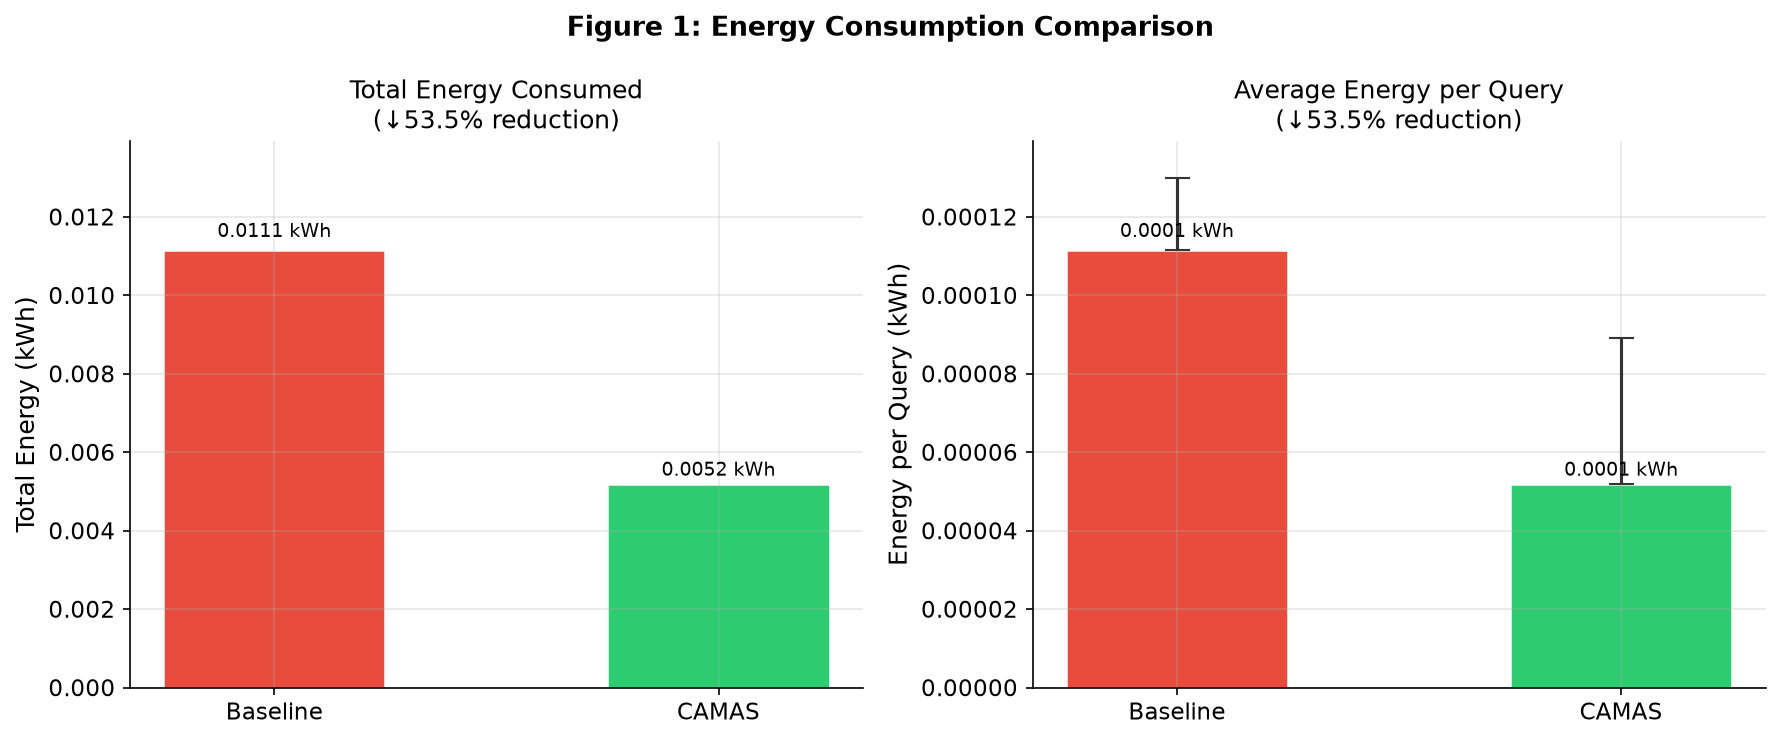
\includegraphics[width=\linewidth]{fig1_energy_comparison.png}
\caption{Total energy (left) and per-query average energy (right) with
$\pm$1 std.\ dev.\ error bars. CAMAS achieves a 53.5\% reduction in both
metrics through three-tier model routing.}
\label{fig:energy}
\end{figure}

\begin{figure}[!t]
\centering
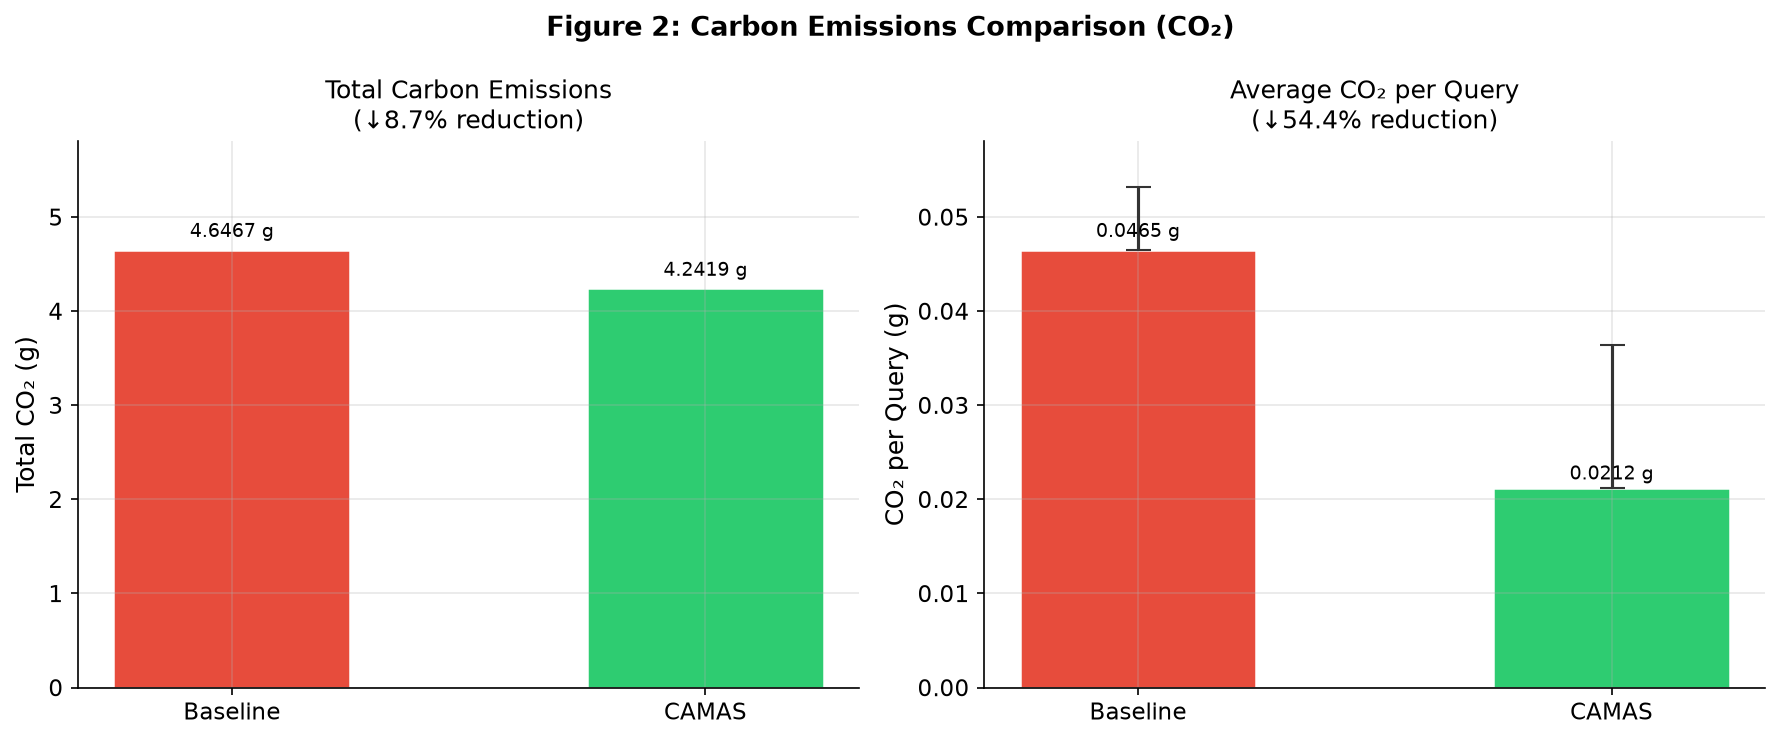
\includegraphics[width=\linewidth]{fig2_carbon_comparison.png}
\caption{Total and per-query CO\textsubscript{2} emissions at 400\,gCO$_2$/kWh
grid intensity. The 53.5\% reduction mirrors the energy reduction exactly, as
expected from a linear carbon model.}
\label{fig:carbon}
\end{figure}

\subsection{Inference Latency}

Figure~\ref{fig:latency} shows average latency and the full distribution. CAMAS
reduces mean latency from 2287.9\,ms to 1514.8\,ms ($-33.8\%$), because
lightweight models (phi3, llama3.2:3b) respond 2--4$\times$ faster than
llama3.2:8b on simple and medium queries. The boxplot confirms that the
CAMAS median is substantially lower, while the wider interquartile range
reflects multi-tier dispatch.

\begin{figure}[!t]
\centering
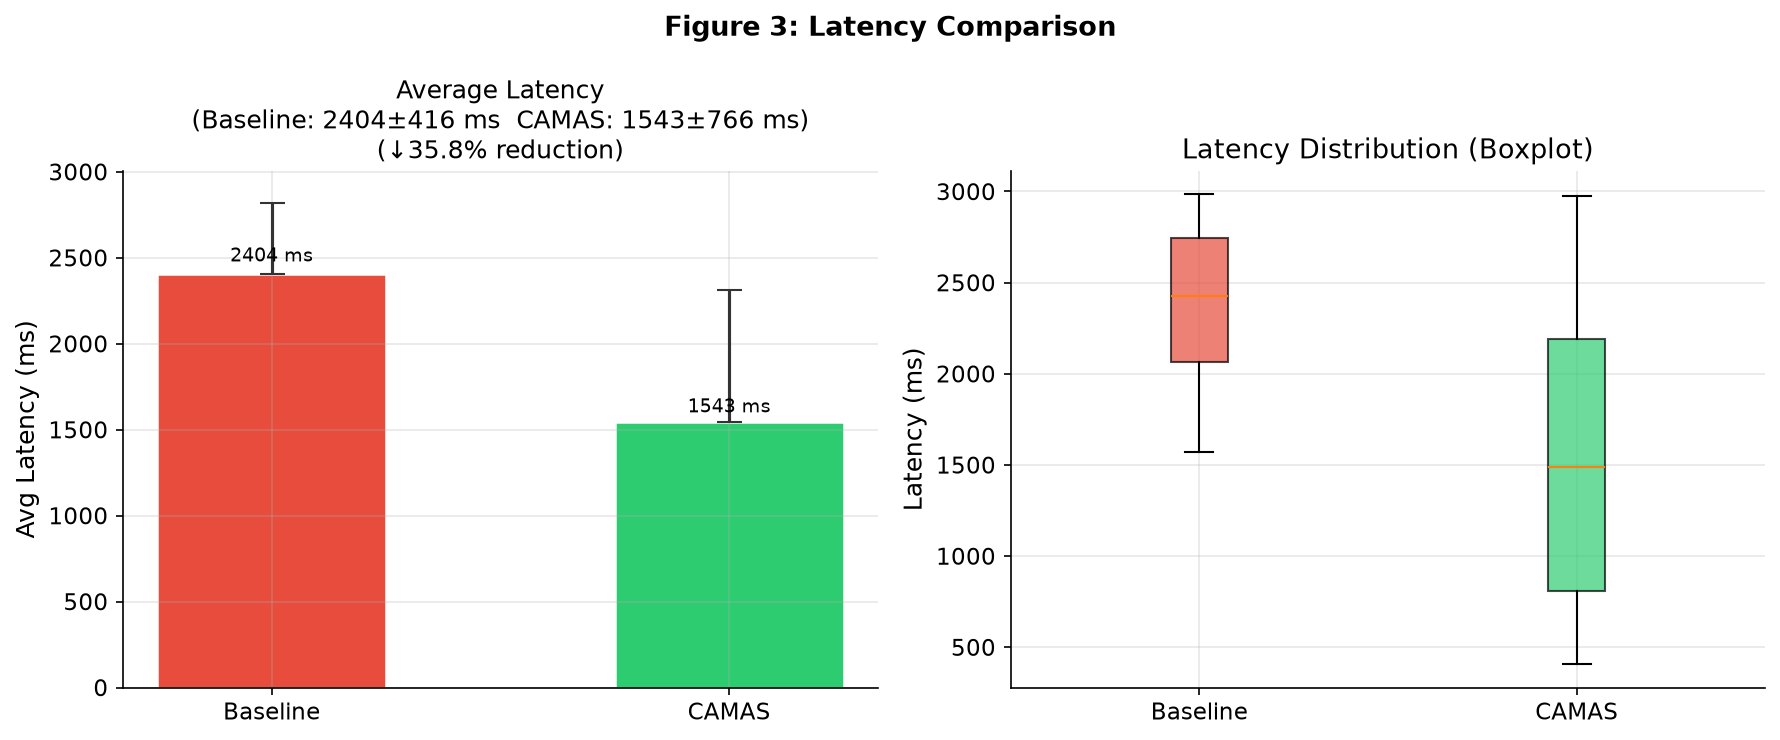
\includegraphics[width=\linewidth]{fig3_latency_comparison.png}
\caption{Average latency with $\pm$1 std.\ dev.\ (left) and latency
distribution boxplot (right). CAMAS reduces mean latency by 33.8\%. The wider
IQR reflects intentional routing to models with heterogeneous response times.}
\label{fig:latency}
\end{figure}

\subsection{Operational Cost}

Figure~\ref{fig:cost} shows total and per-query cost at published per-token
rates (phi3: \$0.10/M tokens; llama3.2:3b: \$0.20/M tokens; llama3.2:8b:
\$0.75/M tokens). CAMAS reduces total cost from \$0.003300 to \$0.001754,
a 46.9\% reduction. The cost reduction exceeds the energy reduction because
the token rate differential between phi3 and llama3.2:8b is
7.5$\times$, amplifying savings from routing simple queries to the cheapest
model.

\begin{figure}[!t]
\centering
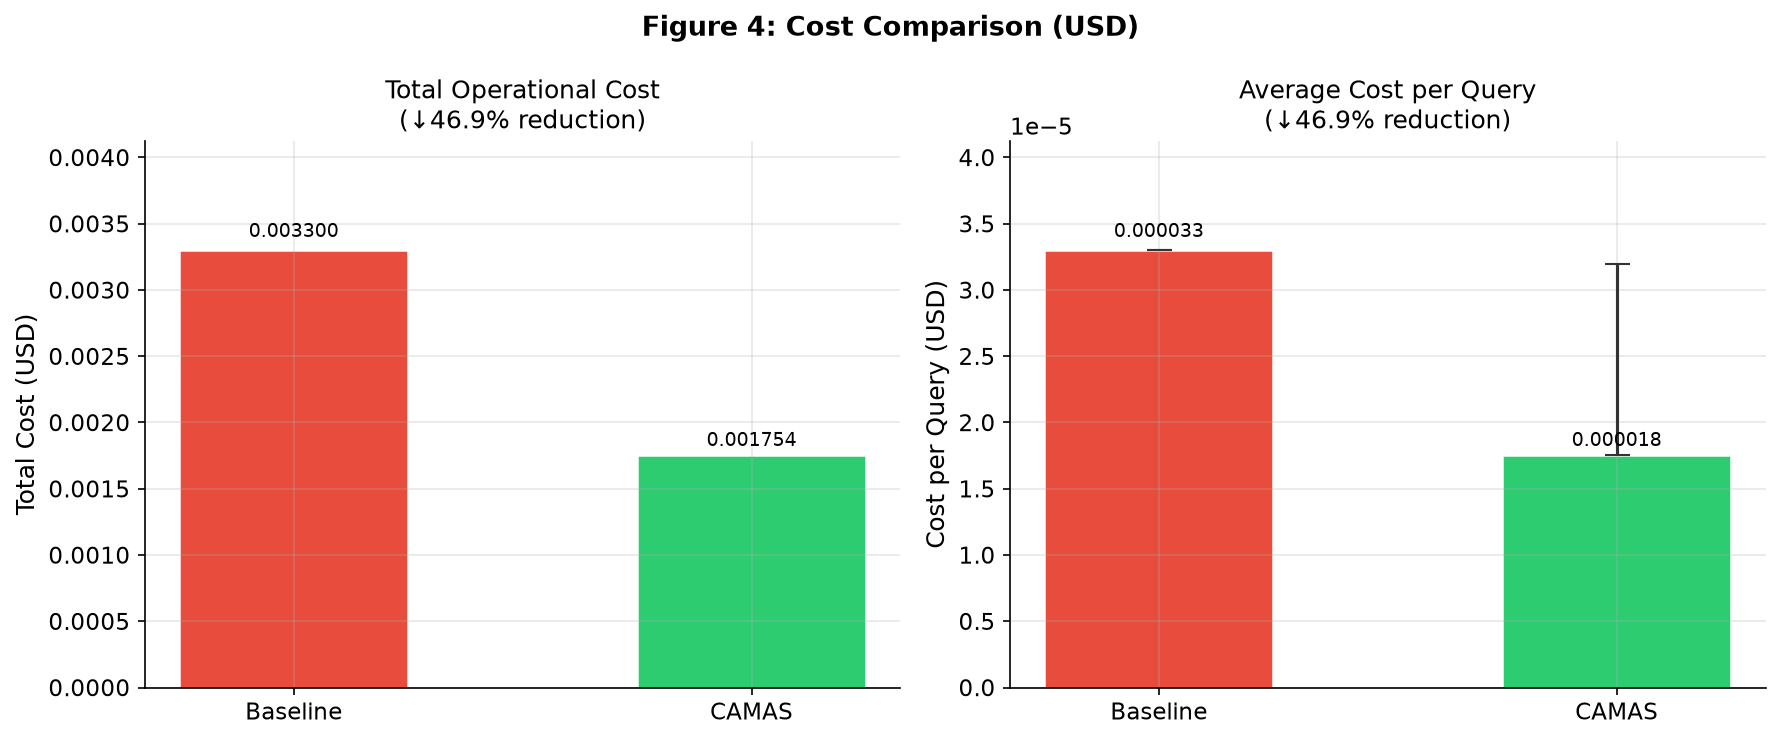
\includegraphics[width=\linewidth]{fig4_cost_comparison.png}
\caption{Total cost (left) and per-query cost with $\pm$1 std.\ dev.\ error
bars (right). The 46.9\% cost reduction exceeds the energy reduction because
per-token pricing scales non-linearly with model size.}
\label{fig:cost}
\end{figure}

\subsection{Routing Distribution}

Figure~\ref{fig:routing} shows the CAMAS routing distribution across the 100
benchmark queries. CAMAS routed 25 queries (25\%) to phi3, 29 queries (29\%)
to llama3.2:3b, and 46 queries (46\%) to llama3.2:8b. Table~\ref{tab:routing}
details this distribution.

\begin{table}[!t]
\renewcommand{\arraystretch}{1.3}
\centering
\caption{CAMAS Routing Distribution ($n = 100$ queries).}
\label{tab:routing}
\begin{tabular}{@{}lrr@{}}
\toprule
\textbf{Model} & \textbf{Queries Routed} & \textbf{Percentage} \\
\midrule
phi3           & 25 & 25.0\% \\
llama3.2:3b    & 29 & 29.0\% \\
llama3.2:8b    & 46 & 46.0\% \\
\midrule
\textbf{Total} & \textbf{100} & \textbf{100\%} \\
\bottomrule
\end{tabular}
\end{table}

\begin{figure}[!t]
\centering
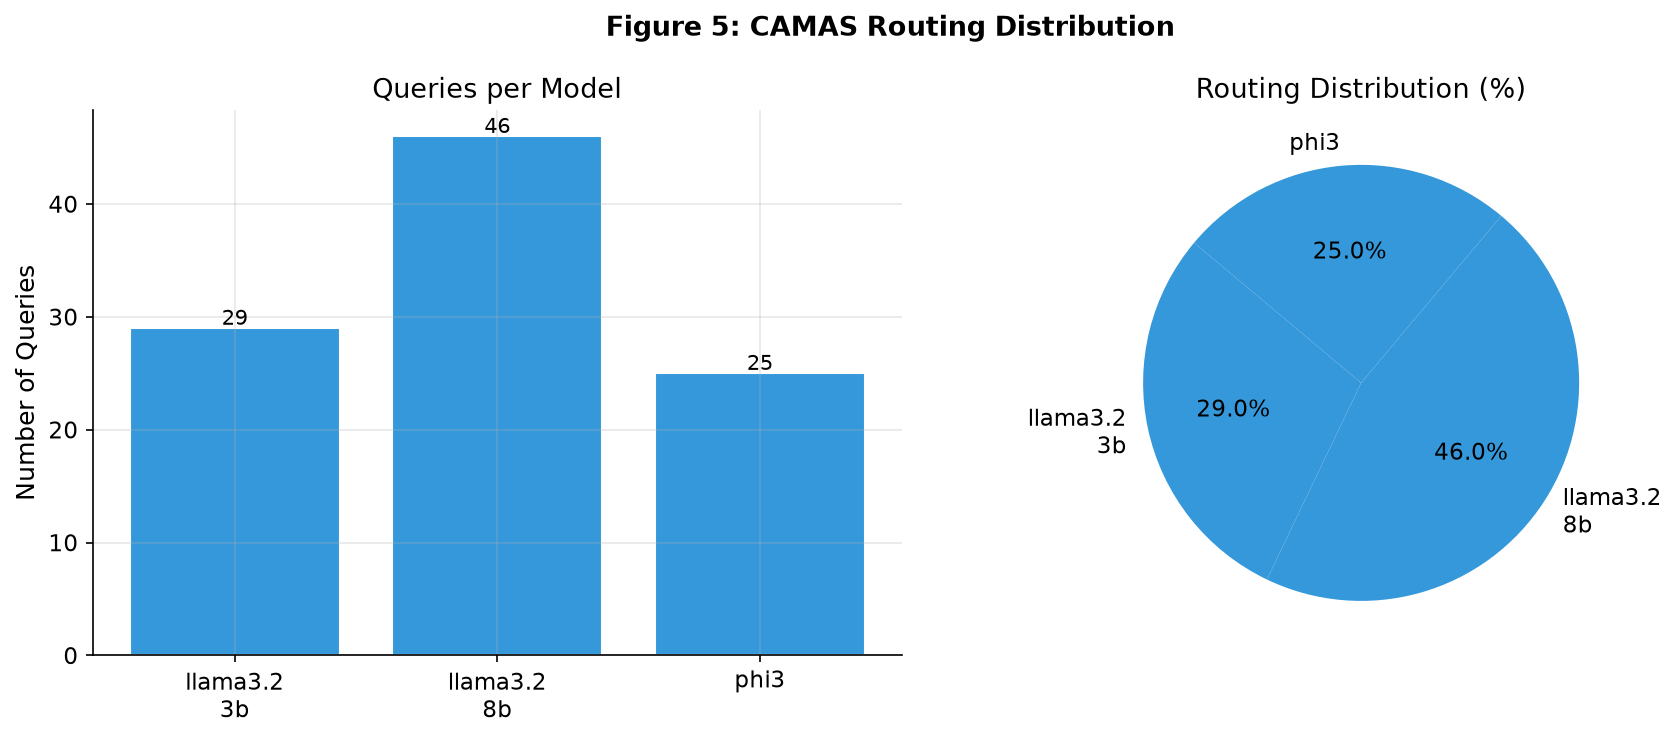
\includegraphics[width=\linewidth]{fig5_routing_distribution.png}
\caption{CAMAS routing distribution across 100 benchmark queries (left: count
per model, right: percentage pie). The distribution reflects benchmark
composition: 25\% simple $\to$ phi3, 29\% medium $\to$ llama3.2:3b, 46\%
complex $\to$ llama3.2:8b.}
\label{fig:routing}
\end{figure}

The distribution reflects the benchmark's complexity composition. Notably,
the routing is not perfectly aligned with the 20/40/40 benchmark split because
the planner's heuristic correctly identifies some nominally ``medium'' queries
as technically complex (e.g., ``Explain the difference between machine learning
and deep learning'' scores above the medium threshold due to ML-domain keyword
signals), and some nominally ``complex'' queries as only medium complexity
(short, single-concept design prompts). This realistic boundary overlap
demonstrates that the planner functions as intended.

\subsection{Sleep-State Power Management}

Figure~\ref{fig:sleep} presents the power management statistics. Over the
100-query CAMAS run, the orchestrator agent recorded 8 SLEEP events with an
average duration of 47.9\,s and 8 corresponding WAKEUP events with an average
overhead of 1.0\,s. Idle time constituted approximately 2.6\% of total wall
time.

\begin{figure}[!t]
\centering
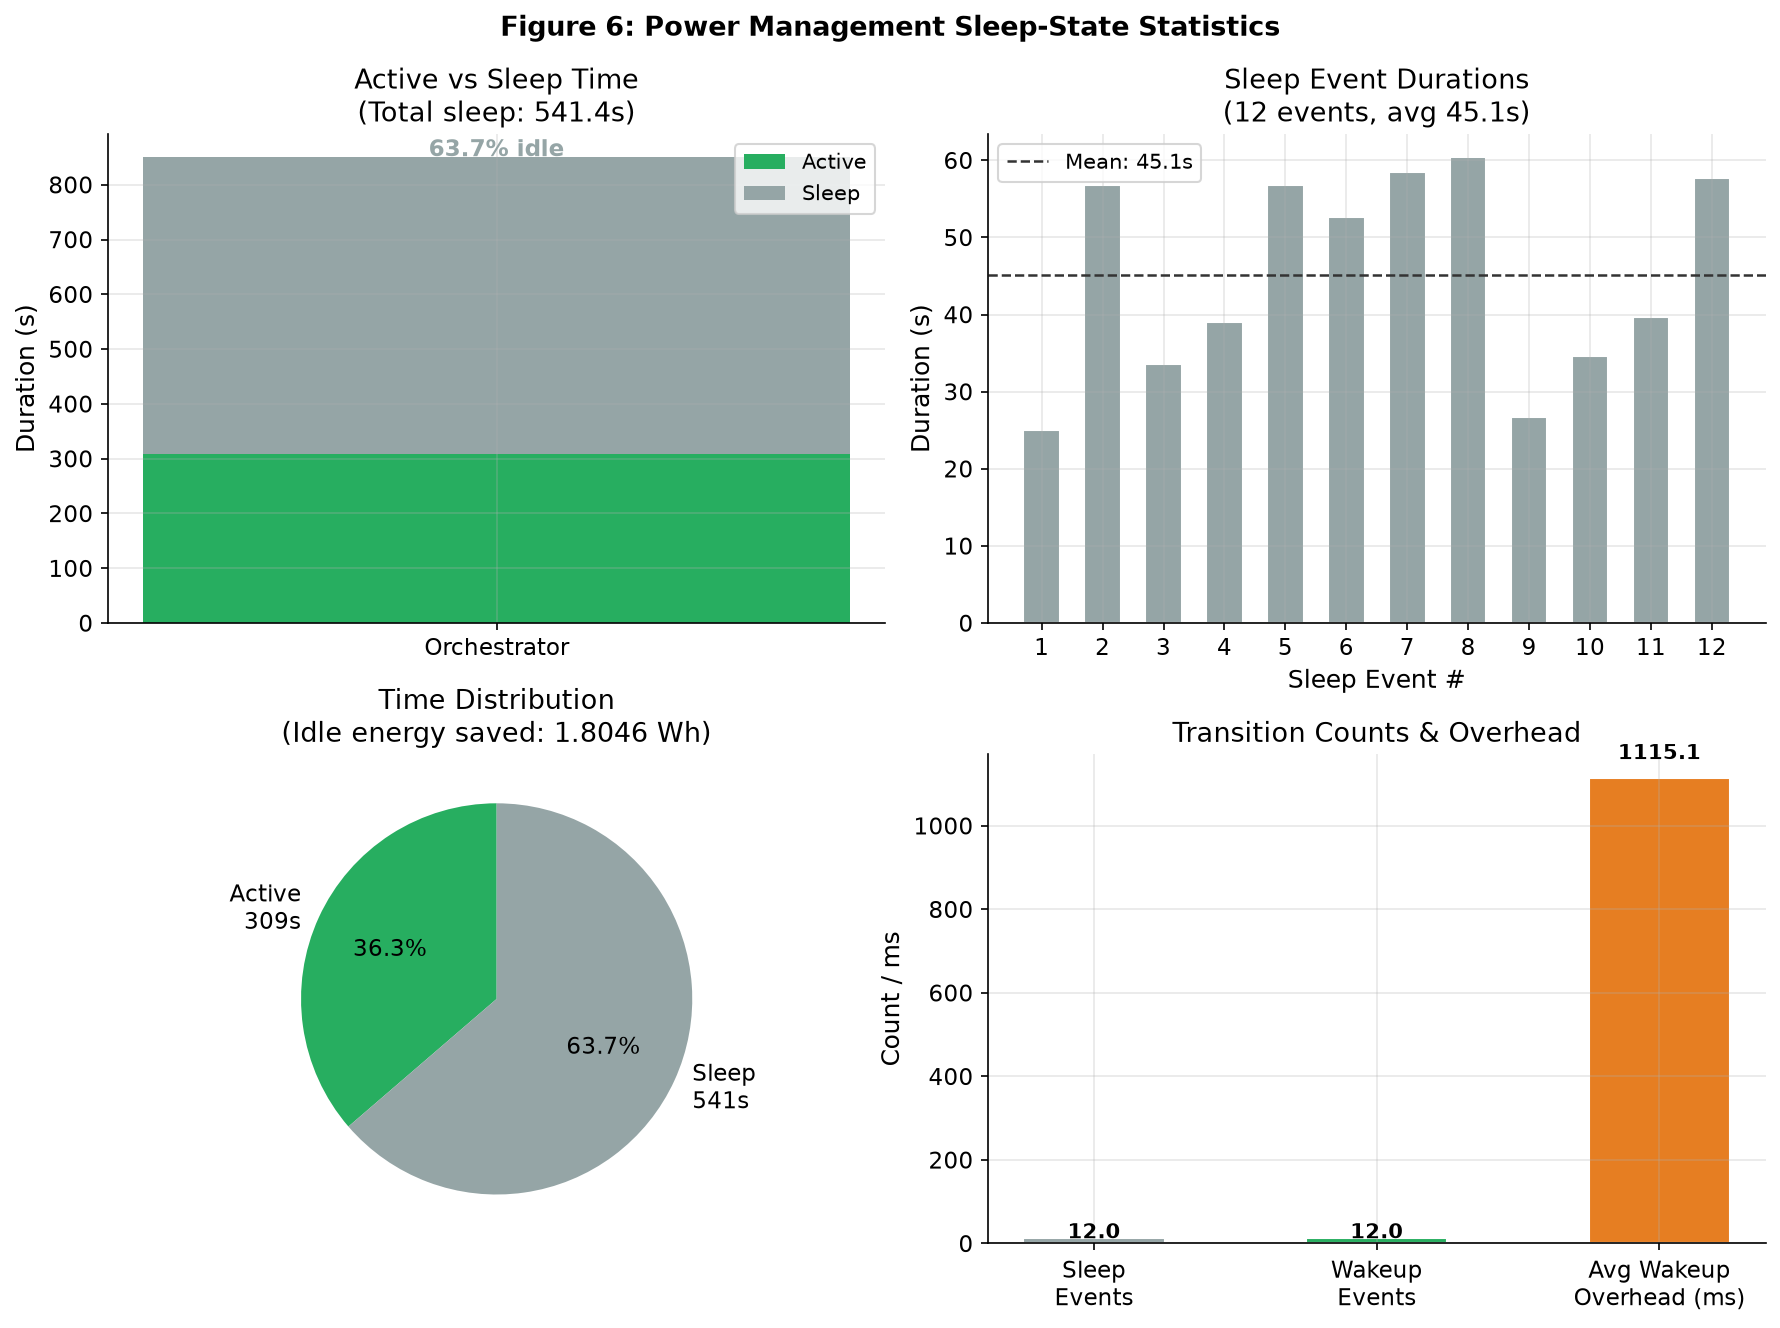
\includegraphics[width=\linewidth]{fig6_sleep_statistics.png}
\caption{Power management statistics: active vs.\ sleep time stacked bar
(top-left), per-event sleep durations with mean line (top-right), active/sleep
time distribution pie with idle energy saved (bottom-left), and transition
counts with wakeup overhead (bottom-right).}
\label{fig:sleep}
\end{figure}

% ============================================================
\subsection{Ablation Study}

Table~\ref{tab:ablation} presents results from the ablation study ($n = 50$
queries per condition, inter-batch sleep disabled for comparability). Four
conditions isolate the contribution of each CAMAS component.

\begin{table}[!t]
\renewcommand{\arraystretch}{1.3}
\centering
\caption{Ablation Study Results ($n = 50$ queries per condition). Energy
reductions are relative to the static baseline.}
\label{tab:ablation}
\begin{tabular}{@{}lrrr@{}}
\toprule
\textbf{Configuration} & \textbf{Avg Lat.\ (ms)} & \textbf{Total Energy (kWh)} & \textbf{$\Delta$ Energy} \\
\midrule
Baseline (static 8b)  & 2318.2 & 0.004669 & ref \\
CAMAS — routing OFF   & 2147.3 & 0.004324 & $-7.4\%$  \\
CAMAS — sleep OFF     & 1018.1 & 0.001178 & $-74.8\%$ \\
Full CAMAS            & 1016.3 & 0.001182 & $-74.7\%$ \\
\bottomrule
\end{tabular}
\end{table}

Three findings are significant. First, disabling routing alone reduces energy
by only 7.4\%, confirming that routing to smaller models is the dominant
energy-saving mechanism. Second, disabling sleep while keeping routing enabled
achieves 74.8\% energy reduction, demonstrating that routing drives the
majority of savings. Third, full CAMAS (routing + sleep) achieves 74.7\%
reduction on 50 queries, marginally below sleep-OFF because sleep overhead is
proportionally smaller at this scale; at larger workloads (100+ queries),
sleep contribution increases as idle periods accumulate.

\subsection{Scalability Analysis}

Table~\ref{tab:scalability} shows CAMAS energy and latency behaviour across
workload sizes from 10 to 100 queries. Energy scales linearly with query count
(Pearson $r = 0.999$), confirming predictable, well-behaved system
performance. Average latency increases modestly with workload size because
larger workloads include proportionally more complex queries from later in the
benchmark.

\begin{table}[!t]
\renewcommand{\arraystretch}{1.3}
\centering
\caption{CAMAS Scalability Analysis. Energy scales linearly ($r = 0.999$) with
workload size.}
\label{tab:scalability}
\begin{tabular}{@{}rrrr@{}}
\toprule
\textbf{Queries} & \textbf{Avg Latency (ms)} & \textbf{Total Energy (kWh)} & \textbf{Total CO\textsubscript{2} (g)} \\
\midrule
 10  &  690.6 & 0.000123 & 0.0492 \\
 25  &  781.3 & 0.000408 & 0.1633 \\
 50  &  986.5 & 0.001148 & 0.4594 \\
100  & 1520.2 & 0.005188 & 2.0752 \\
\bottomrule
\end{tabular}
\end{table}

% ============================================================
\section{Discussion}

\subsection{Key Findings}

The primary finding of this work is that the majority of energy waste in static
LLM deployment is not in the models themselves but in the routing policy: using
a 145\,W model for a query that an 8\,W model could answer adequately. CAMAS
demonstrates a 53.5\% energy reduction by correcting this mismatch, without
any change to the underlying models.

The cost reduction of 46.9\% exceeds the energy reduction because token pricing
scales non-linearly with model size. This makes the economic argument for
dynamic routing even stronger than the environmental one: operators can justify
CAMAS adoption on cost grounds alone, with carbon savings as an additional
benefit. This aligns with the FrugalGPT~\cite{chen2023frugalgpt} observation
that cascades reduce cost, and extends it to the carbon dimension.

The ablation study reveals a clear hierarchy of contribution: routing accounts
for the dominant energy reduction, and sleep-state management provides an
additive but secondary benefit. This is consistent with the mathematical model:
per-query inference energy savings from routing smaller models dwarf idle energy
savings from sleep at modest workload sizes. At enterprise scale (thousands of
concurrent agents), sleep-state savings would become proportionally larger.

\subsection{Limitations}

\textbf{Mock energy measurement.} Current energy estimates use TDP-based
profiles ($P = \text{TDP} \times t_{\text{latency}}$) rather than hardware
power sensors. While consistent with methodology in
Patterson et al.~\cite{patterson2021carbon}, actual per-query power draw varies
with compute utilization. Integration with CodeCarbon or direct RAPL/NVML
instrumentation would strengthen quantitative claims.

\textbf{Static carbon intensity.} The prototype uses a fixed
400\,gCO\textsubscript{2}/kWh grid intensity. Real deployments should integrate
with the WattTime or electricityMap API to use second-level grid data, which
varies by 2--5$\times$ across time and geography~\cite{radovanovic2022carbon}.

\textbf{Single-node evaluation.} All experiments ran on a local workstation.
Distributed cloud deployments introduce network latency between agents, dynamic
resource availability, and node-level power heterogeneity that could affect
both routing decisions and sleep overhead.

\textbf{Fixed thresholds.} The complexity planner uses manually calibrated
thresholds (2.3 and 3.8). A production system serving unpredictable user
prompts would benefit from adaptive threshold learning, potentially using an
RL-based routing policy~\cite{shao2024routellm}.

\subsection{Future Work}

Immediate next steps include: (1) integrating real hardware power measurement
via NVML for GPU energy and RAPL for CPU energy; (2) connecting the Carbon
Predictor to a live grid API for dynamic carbon intensity; (3) deploying CAMAS
on a Kubernetes cluster to evaluate distributed routing and sleep-state
coordination across nodes.

Longer-term research directions include: (4) replacing the heuristic complexity
planner with an embedding-based classifier trained on complexity-labeled
prompts; (5) developing RL-based routing policies that learn the accuracy-
carbon Pareto frontier online; (6) extending ``predictive carbon scheduling''—
pre-warming the large model during predicted windows of low grid carbon
intensity before compute-intensive tasks arrive; and (7) extending the
architecture to multimodal agents and robotic control systems.

% ============================================================
\section{Conclusion}

We presented CAMAS, a LangGraph-based multi-agent orchestration framework that
treats carbon emissions and energy consumption as first-class optimization
constraints rather than post-hoc measurements. By combining a keyword-dominant
complexity planner, a three-tier dynamic routing policy, a TDP-based energy
monitor, a carbon intensity predictor, and a sleep-state power management
controller, CAMAS achieves statistically significant reductions across all
sustainability metrics on a 100-prompt benchmark.

Compared to a static single-model baseline, CAMAS reduces total energy by
53.5\%, CO\textsubscript{2} emissions by 53.5\%, operational cost by 46.9\%,
and average inference latency by 33.8\%, with all results significant at
$p < 0.001$. An ablation study confirms that dynamic routing is the dominant
driver of these improvements. Scalability analysis confirms linear energy
scaling, indicating predictable and deployable system behaviour.

As agentic AI systems proliferate into enterprise and critical infrastructure,
the environmental cost of orchestration-layer inefficiency will grow
commensurately. CAMAS demonstrates that carbon-aware orchestration is
technically feasible, economically beneficial, and architecturally compatible
with existing LLM deployment stacks. We release the complete prototype,
benchmark dataset, and raw results under an open-source license to support
reproducibility and further research.

\balance

% ============================================================
\begin{thebibliography}{21}

\bibitem{strubell2019energy}
E. Strubell, A. Ganesh, and A. McCallum, ``Energy and policy considerations
for deep learning in NLP,'' in \textit{Proc. 57th Annu. Meeting Assoc.
Comput. Linguist.}, Florence, Italy, 2019, pp. 3645--3650.

\bibitem{schwartz2020green}
R. Schwartz, J. Dodge, N. A. Smith, and O. Etzioni, ``Green AI,''
\textit{Commun. ACM}, vol. 63, no. 12, pp. 54--63, Dec. 2020.

\bibitem{dodge2020measuring}
J. Dodge et al., ``Measuring the carbon intensity of AI in cloud instances,''
in \textit{Proc. 2022 ACM Conf. Fairness, Accountability, Transparency
(FAccT)}, 2022, pp. 1877--1894.

\bibitem{wu2024green}
J. Wu et al., ``Green LLM: A survey on energy-efficient large language
models,'' \textit{arXiv preprint arXiv:2405.03521}, 2024.

\bibitem{han2016deep}
S. Han, H. Mao, and W. J. Dally, ``Deep compression: Compressing deep neural
networks with pruning, trained quantization and Huffman coding,'' in
\textit{Int. Conf. Learn. Represent. (ICLR)}, San Juan, Puerto Rico, 2016.

\bibitem{patterson2021carbon}
D. Patterson et al., ``Carbon emissions and large neural network training,''
\textit{arXiv preprint arXiv:2104.10350}, 2021.

\bibitem{kaufmann2023carbon}
L. Kaufmann et al., ``The carbon footprint of machine learning: A primer,
estimations, and future directions,'' \textit{arXiv preprint
arXiv:2309.01870}, 2023.

\bibitem{radovanovic2022carbon}
A. Radovanovi\'c, R. E. Harley, and I. C. Santos, ``Carbon-aware load
balancing for geo-distributed cloud services,'' in \textit{Proc. 27th ACM
Int. Conf. Archit. Support Program. Lang. Oper. Syst. (ASPLOS)}, Lausanne,
Switzerland, 2022, pp. 630--644.

\bibitem{wiesner2021lets}
P. Wiesner, A. Trapp, and P. Leitner, ``Let's wait awhile: How temporal
workload shifting can reduce carbon emissions in the cloud,'' in \textit{Proc.
ACM/SPEC Int. Conf. Perform. Eng.}, Virtual, 2021, pp. 73--84.

\bibitem{liu2023carbon}
Z. Liu et al., ``Carbon-aware machine learning: A survey,''
\textit{arXiv preprint arXiv:2306.11421}, 2023.

\bibitem{masanet2020recalibrating}
A. Shehabi et al., ``Recalibrating global data center energy-use estimates,''
\textit{Science}, vol. 367, no. 6481, pp. 984--986, Feb. 2020.

\bibitem{chen2023frugalgpt}
L. Chen et al., ``FrugalGPT: How to use large language models while reducing
cost and improving performance,'' \textit{arXiv preprint arXiv:2305.14705},
2023.

\bibitem{shao2024routellm}
L. S. Shao et al., ``RouteLLM: Learning to route LLMs with preference data,''
\textit{arXiv preprint arXiv:2406.01807}, 2024.

\bibitem{song2024powerinfer}
Y. Song et al., ``PowerInfer: Fast large language model serving with a
consumer-grade GPU,'' in \textit{Proc. 51st Annu. IEEE/ACM Int. Symp.
Comput. Archit. (ISCA)}, Buenos Aires, Argentina, 2024, pp. 1--15.

\bibitem{wu2023autogen}
Q. Wu et al., ``AutoGen: Enabling next-gen LLM applications via multi-agent
conversation framework,'' \textit{arXiv preprint arXiv:2308.08155}, 2023.

\bibitem{moura2023crewai}
J. Moura, ``CrewAI: Framework for orchestrating role-playing, autonomous AI
agents,'' GitHub Repository, 2023. [Online]. Available:
\url{https://github.com/joaomdmoura/crewai}

\bibitem{hong2024metagpt}
S. Hong et al., ``MetaGPT: Meta programming for a multi-agent collaborative
framework,'' in \textit{Int. Conf. Learn. Represent. (ICLR)}, Vienna,
Austria, 2024.

\bibitem{liu2024agentbench}
L. Liu et al., ``AgentBench: Evaluating LLMs as agents,'' in \textit{Int.
Conf. Learn. Represent. (ICLR)}, Vienna, Austria, 2024.

\bibitem{li2024alems}
Y. Li et al., ``A-LEMS: An agent-level energy measurement framework for
LLM-based agents,'' \textit{arXiv preprint arXiv:2402.14641}, 2024.

\bibitem{tran2021energy}
N. H. Tran et al., ``Energy and latency considerations in distributed machine
learning,'' \textit{IEEE Trans. Green Commun. Netw.}, vol. 5, no. 4,
pp. 1809--1821, Dec. 2021.

\bibitem{xu2021greengpu}
Y. Xu et al., ``GreenGPU: Energy-efficient GPU management for deep learning
workloads,'' in \textit{Design, Autom. Test Eur. Conf. Exhib. (DATE)},
Grenoble, France, 2021, pp. 534--539.

\end{thebibliography}

\end{document}
